---
id: tkz-euclide-ejemplo-55
title: "Triángulo equilátero"
description: "Creación de un triángulo equilátero"
keywords: [angulo,triangulo,equilatero,taller2]
tags: [tkzDefTriangle,tkzMarkSegments,tkzMarkAngles,tkzFillAngles,tkzDrawPolygon]
sort: 55
---
\documentclass[tikz,border=2mm]{standalone}
\usepackage{tkz-base}
\usepackage{tkz-euclide}

\begin{document}
    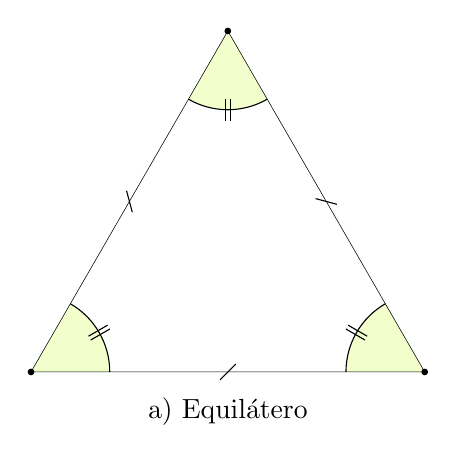
\begin{tikzpicture}
        % Paso 1: Define los puntos de la base AB
        \tkzDefPoint(1,1){A}
        \tkzDefPoint(6,1){B}

        % Paso 2: Define el triángulo equilatero por △ABC
        % y obtienes el tercer punto C.
        \tkzDefTriangle[equilateral](A,B)
             \tkzGetPoint{C}

        % Paso 3: Marca los segments congruentes
        \tkzMarkSegments[mark=s|](A,B B,C C,A)
        
        % Paso 4: Rellena ángulos y marca los congruentes
        \tkzFillAngles[fill=lime!20](B,A,C C,B,A A,C,B) % ∠BAC, ∠CBA, ∠ACB
        \tkzMarkAngles[mark=||](B,A,C C,B,A A,C,B) % ∠BAC, ∠CBA, ∠ACB

        % Paso 5: Dibuja los puntos y el polígono
        \tkzDrawPoints(A,B,C)
        \tkzDrawPolygon(A,B,C)

        % Paso 6: Agrega una leyenda al gráfico
        \tkzText(3.5,0.5){a) Equilátero}        
    \end{tikzpicture}
\end{document}